% ──────────────────────────────────────────────────────────────────────
% Comparative Study Research Paper (double-blind submission)
% Springer LNCS proceedings format (llncs.cls, Version 2.25 of 2026/09/03)
%
% Compile with:
%   pdflatex paper
%   bibtex   paper
%   pdflatex paper
%   pdflatex paper
% ──────────────────────────────────────────────────────────────────────
\documentclass[runningheads]{llncs}
%
\usepackage[T1]{fontenc}
% T1 fonts will be used to generate the final print and online PDFs,
% so please use T1 fonts in your manuscript whenever possible.
%
% The reference LNCS template selects Times Roman via the newtx fonts.
% Fall back to a Times (ptm) text face where newtx is unavailable,
% so the manuscript remains compilable on any TeX installation.
\IfFileExists{newtxtext.sty}{%
  \usepackage{newtxtext}       % selects Times Roman as basic font
  \usepackage[varvw]{newtxmath}
}{%
  \renewcommand{\rmdefault}{ptm}% Times Roman text fallback
}
\usepackage{graphicx}
\usepackage{array}
\usepackage{url}
\usepackage{amsmath}
\emergencystretch=1.5em       % avoid ugly overfull lines in justified text
%
% If you use the hyperref package, please uncomment the following two lines
% to display URLs in blue roman font according to Springer's eBook style:
%\usepackage{color}
%\renewcommand\UrlFont{\color{blue}\rmfamily}
%\urlstyle{rm}
%
\begin{document}
%
\title{A Comparative Study of Self-Supervised and Spectrogram-Based
Models for Cross-Corpus Speech Dysfluency Detection}
%
\titlerunning{A Comparative Study}
% If the paper title is too long for the running head, you can set
% an abbreviated paper title here.
%
\author{Anonymous}
%
\authorrunning{Anonymous}
% Anonymous submission: author details, affiliations, and contact
% information are withheld for double-blind review.
%
\institute{}           % suppressed for double-blind review
%
\maketitle              % typeset the header of the contribution
%
\begin{abstract}
Stuttering is a speech disorder that manifests as involuntary repetitions,
prolongations, and blocks, impacting communication and quality of life, and it
affects roughly 1\% of the adult population and up to 5\% of
children~\cite{yairi2009childhood}. Automated detection of dysfluency events is
challenging due to the subtle acoustic signatures and strong class imbalance
across dysfluency types (prolongation, block, sound repetition, word
repetition, interjection). This paper presents an end-to-end speech dysfluency
classification system and compares seven experimental configurations spanning
two representation families: self-supervised waveform-based models built on
Wav2Vec~2.0 (five independent binary classifiers and a shared-backbone
multitask variant) and compact mel-spectrogram CNN models (pooled,
single-head, LSTM-augmented, and transformer-augmented). All models are
evaluated on a merged corpus of 37,087 clips drawn from SEP-28K, UCLASS, and
Project Boli (36,674 usable after removing empty audio) under two protocols:
an in-distribution clip-level held-out evaluation and a speaker-independent
cross-corpus evaluation on Project Boli (unseen speakers, languages, and
recording conditions). Under the clip-level protocol, the five-binary
Wav2Vec 2.0 configuration achieves the highest measured macro F1 (0.5704 at
validation-tuned thresholds), while the shared-backbone multitask variant
follows closely (0.5557) using ${\approx}4.9\times$ fewer parameters than five
separate classifiers; however, this protocol shares
speakers between training and test, so these results are not
speaker-independent. On the 53-clip speaker-independent Boli set, no
configuration exceeds a trivial all-positive baseline (macro F1 $=0.55$):
apparent cross-corpus F1 differences are dominated by class base rates and by
threshold/operating-point drift on the distribution-shifted set rather than by
ranking quality. Under the threshold-free metrics the ordering is reversed,
with the two task-adapted Wav2Vec2 configurations ranking Boli clips best
(macro AUROC ${\approx}0.62$) while the CNN configurations sit around chance
(${\approx}0.47$--$0.52$). These results demonstrate
that tuned-F1 comparisons on a small imbalanced external corpus do not
reliably measure cross-corpus generalization; we therefore treat ranking-based
metrics and per-class analysis as the primary evidence, discuss the trade-offs
between representation capacity and generalization, and frame the observed
generalization gap as an open hypothesis. We report per-class precision,
recall, F1, AUROC, and AUPRC across all five dysfluency types. All results are
single-seed point estimates and should be interpreted accordingly.

\keywords{Speech dysfluency detection \and stuttering classification \and
Wav2Vec 2.0 \and multitask learning \and cross-corpus evaluation \and
speaker-independent evaluation.}
\end{abstract}
%
%
%
\section{Introduction}
Stuttering affects approximately 1\% of the global adult population and up to
5\% of children~\cite{yairi2009childhood}. Characterized by involuntary
repetitions of sounds, syllables, or words (sound repetitions and word
repetitions), abnormal prolongations of speech sounds (prolongations), and
involuntary pauses or stops in speech flow (blocks), it impacts the
psychosocial well-being of affected individuals~\cite{yairi2009childhood}.
Traditional assessment by speech-language pathologists (SLPs) relies on
subjective auditory perception and visual inspection of waveforms, a process
that is time-consuming, prone to inter-rater variability, and unscalable for
large populations; this has motivated a large body of work on automatic
stuttering identification~\cite{sheikh2022review}.

Recent advances in self-supervised speech representation learning, particularly
Wav2Vec 2.0~\cite{baevski2020wav2vec}, have achieved strong performance on
downstream speech classification tasks by learning contextualized representations
from raw audio. Applying such models to stuttering detection presents challenges:
the five dysfluency types have different acoustic signatures, and severe class
imbalance exists (most speech segments are fluent)~\cite{lea2021sep28k}.

This paper makes the following contributions:
\begin{itemize}
\item We present a modular system for speech dysfluency
classification, supporting five dysfluency types: prolongation, block, sound
repetition, word repetition, and interjection.
\item We conduct a systematic comparative study of seven experimental
configurations across two representation families---self-supervised waveform
models (Wav2Vec 2.0) and mel-spectrogram CNN models---on a merged multi-corpus
dataset.
\item We evaluate under two complementary protocols: a clip-level in-distribution
held-out split and a speaker-independent cross-corpus held-out set (Project
Boli), and we report both macro and per-class metrics including AUPRC.
\item We analyze per-class performance across all five dysfluency types, showing
that interjection achieves the highest F1 among the evaluated classes while block
is the most challenging. We further demonstrate that tuned-F1 results on the
small external Boli set are dominated by class base rates and operating-point
drift---no configuration beats a trivial all-positive baseline there---so
cross-corpus claims must be evaluated with threshold-free metrics, and we
articulate the open hypotheses that surround the observed
in-distribution/cross-corpus generalization gap.
\end{itemize}

The remainder of this paper is organized as follows: Section~\ref{sec:related}
reviews related work, Section~\ref{sec:arch} describes the system architecture,
Section~\ref{sec:setup} details the experimental setup, Section~\ref{sec:results}
presents results and discussion, and Section~\ref{sec:conclusion} concludes.

% ── II. RELATED WORK ─────────────────────────────────────────────────
\section{Related Work}
\label{sec:related}

\subsection{Traditional Approaches}
Early stutter detection systems relied on handcrafted acoustic features,
including jitter, shimmer, spectral flux, and formant trajectories, combined with
classical classifiers such as Support Vector Machines (SVMs), Hidden Markov
Models (HMMs), and Gaussian Mixture Models (GMMs)~\cite{sheikh2022review}.
These methods achieved reasonable accuracy on controlled datasets but generalized
poorly across speakers, accents, and recording conditions due to the limited
representational capacity of handcrafted features.

\subsection{Deep Learning Methods}
The introduction of end-to-end deep learning approaches removed the need for
manual feature engineering. Convolutional Neural Networks (CNNs) operating on
mel-spectrograms, combined with recurrent layers, showed early promise for
multi-type dysfluency
detection~\cite{kourkounakis2020detecting}. Recurrent Neural Networks (RNNs),
Long Short-Term Memory (LSTM) networks, and time-delay neural networks were
applied to capture temporal dependencies in speech
signals~\cite{kourkounakis2020detecting,sheikh2021stutternet}. More recently,
transformer-based architectures, particularly Wav2Vec
2.0~\cite{baevski2020wav2vec}, have achieved strong results on speech processing
tasks by learning contextualized representations from raw audio through
self-supervised pre-training on large unlabeled corpora.

\subsection{Self-Supervised Speech Representation Models}
Self-supervised pre-training has become the dominant paradigm for speech
representation learning. Wav2Vec 2.0~\cite{baevski2020wav2vec} learns
contextualized speech representations by contrasting quantized latent speech
units and masking spans of the input waveform, and it generalizes across
languages when pre-trained on multilingual data
(XLSR-53~\cite{conneau2021xlsr}). HuBERT~\cite{hsu2021hubert} instead predicts
masked hidden units obtained from an offline clustering step and has been shown
to capture strong segmental and suprasegmental characteristics of speech.
XLS-R~\cite{babu2022xlsr} scales the Wav2Vec 2.0 objective to 128 languages and
436K hours of speech. WavLM~\cite{chen2022wavlm} augments masked prediction with
denoising objectives to improve robustness on full-stack speech-processing
downstream tasks. A consistent property of these models is that their embeddings
encode both linguistic content and paralinguistic attributes such as speaker
identity and recording condition; the amount of such non-lexical information
carried in the representation is a design trade-off that is central to our
analysis of cross-corpus generalization.

\subsection{Wav2Vec2-Based Stutter Detection}
Bayerl et al.~\cite{bayerl2022multi} applied Wav2Vec2 to multi-task stuttering
detection on FluencyBank, achieving macro F1 scores in the range of 0.56--0.63
across five dysfluency types. On the standardized SEP-28k-E partition, published
state-of-the-art results reach per-class F1 values that vary significantly by
dysfluency type (e.g., interjection: 0.78, prolongation: 0.53, block: 0.30,
as reported by Su\v{s}ac et al.~\cite{susac2026stuttmil} for the leading
baselines). These works established Wav2Vec2 as a strong backbone for stutter
detection but focused on classification within a single corpus without systematic
architectural comparison or cross-corpus evaluation.

\subsection{Stuttering and Dysfluency Datasets}
Several stuttering corpora have become available in recent years. SEP-28K
was introduced by Lea et al.~\cite{lea2021sep28k} from publicly available
podcasts of people who stutter, with clip-level majority-vote labels for five
dysfluency types. The same authors released a compatible re-annotation of the
adults-who-stutter portion of FluencyBank, a corpus of transcribed monologue
and dialogue speech~\cite{bernsteinratner2018fluencybank}; together these two
sources provide the 32,321 SEP-28K-format clips used here. UCLASS,
a corpus of stuttered speech from therapy sessions~\cite{howell2009uclass},
provides 4,712 additional clips in SEP-28K format. Project Boli~\cite{boli2025}
is a recent multilingual, multi-accent corpus with word-level dysfluency
annotations in five Indian languages. These datasets differ
in speakers, languages, recording conditions, and annotation granularity
(clip-level versus word-level), which makes cross-corpus generalization difficult
to assess and rarely tested.

\subsection{Cross-Corpus and Speaker-Independent Evaluation}
Prior work has largely evaluated on a single dataset (either SEP-28K or
FluencyBank), making it difficult to assess cross-corpus generalization. A system
trained on one corpus may overfit its speakers, accents, and recording
conditions; evaluating on held-out speakers from the same corpus only partially
reveals this when speakers overlap across splits. Reporting a speaker-independent
protocol (no speaker in more than one split) and a cross-corpus protocol (an
entirely separate corpus) is therefore important for realistic performance
estimates. We follow this reasoning and evaluate all seven configurations both
in-distribution (clip-level) and cross-corpus on Boli, whose speakers, languages,
and recordings are fully disjoint from training.

% ── III. SYSTEM ARCHITECTURE ─────────────────────────────────────────
\section{System Architecture}
\label{sec:arch}

The system comprises a classification pipeline that identifies which dysfluency
types are present in speech audio. The pipeline builds on a common preprocessing
module and exposes models through a unified model registry API.

\subsection{Data Pipeline}
The system integrates three publicly available stuttering datasets:
\begin{itemize}
\item \emph{SEP-28K}~\cite{lea2021sep28k}: 32,321 clips annotated for five
dysfluency types (28,177 podcast clips plus a 4,144-clip FluencyBank
re-annotation), with TSV-format labels.
\item \emph{UCLASS}~\cite{howell2009uclass}: 4,712 clips in SEP-28K format, sourced
from stuttering therapy sessions.
\item \emph{Project Boli}~\cite{boli2025}: 54 clips with word-level dysfluency
annotations and timestamps, recorded by speakers of five Indian languages (Hindi,
Marathi, Telugu, Bengali, and Assamese).
\end{itemize}

Table~\ref{tab:datasets} summarizes their key properties. The three datasets are
merged into a unified corpus of 37,087 clips with per-clip interval CSVs recording
dysfluency events as \texttt{(start\_sec, end\_sec, type)} tuples. Clips with
missing or header-only (empty) audio files are removed, leaving 36,674 usable
clips. An 80/10/10 random split (seed 42) assigns 29,296 training clips, 3,662
validation clips, and 3,716 test clips, where the validation and test splits
contain clips from SEP-28K and UCLASS plus the Boli clips described below.
To guarantee an honest cross-corpus
evaluation, all Project Boli clips are pinned to the test split and never appear
in the training or validation splits. Audio is resampled to 16~kHz mono,
DC-removed, peak-normalized, silence-trimmed, and padded/truncated to a maximum of
3 seconds.

\begin{table}[t]
\caption{Source corpora and their integration into the merged corpus.}
\label{tab:datasets}
\centering
\small
\setlength{\tabcolsep}{4pt}
\begin{tabular}{>{\raggedright\arraybackslash}p{1.6cm}rl>{\raggedright\arraybackslash}p{2.4cm}>{\raggedright\arraybackslash}p{2.6cm}}
\hline
Dataset & Clips & Language(s) & Annotation & Role\\
\hline
SEP-28K & 32,321 & English & clip-level TSV, majority vote & train/val/test\\
UCLASS & 4,712 & English & clip-level TSV & train/val/test\\
Boli & 54 & 5 Indian languages & word-level intervals & test only\\
\hline
\end{tabular}
\end{table}

\subsubsection{Annotation harmonization.}
The three corpora use different annotation conventions, which we map onto a common
set of five binary clip-level labels (prolongation, block, sound repetition, word
repetition, interjection). SEP-28K labels are adopted as-is: a clip is positive
for a dysfluency type if at least two annotators marked it
(\texttt{SEP28K\_MIN\_VOTES} = 2). UCLASS provides one label set per clip in the
same five classes; because each clip is a 3-s window centered on the stutter
event, each present label is materialized as a weak interval centered at 1.5~s
into the clip. Project Boli provides word-level tokens annotated with the labels
\emph{B} (block), \emph{PR} (prolongation), \emph{SR} (sound repetition), \emph{WR}
(word repetition), and \emph{IN} (interjection); these are mapped through a fixed
code table to the same five classes, and a clip is labeled positive for a class if
any of its annotated words carries that class. Thus all downstream models consume
identical five-dimensional binary targets regardless of the original corpus.

\subsubsection{The 3-second window.}
SEP-28K clips are natively 3~s long, so a maximum window of 3~s is the natural
budget for the classification task and matches the predominant corpus. For UCLASS,
whose clips are 3-s windows centered on a stutter event, the window preserves the
event of interest. Because classification is clip-level, an event whose acoustic
extent crosses the window boundary does not alter the training target: the
clip-level label only records presence or absence. This is not the case for
temporal localization, which is out of scope here. Two caveats apply. First,
aggressive silence trimming followed by zero-padding to 3~s can place leading or
trailing speech at the window edges, discarding some prosodic context. Second,
for blocks---which manifest as silent or tenuous pauses---the fixed window and the
trimming may suppress the very pause that defines the event when it falls near a
boundary. We return to this in the discussion of per-class results.

\subsection{Classification Pipeline}

\subsubsection{Five Independent Binary Classifiers.}
Each dysfluency type is handled by a separate binary classifier built on
\texttt{facebook/wav2vec2-base} (94,569,090 parameters per classifier, including a
${\approx}0.2$M-parameter classification head on top of the 94.37M-parameter
backbone). The architecture follows a sequence-classification formulation: raw
audio $\rightarrow$ Wav2Vec2 encoder $\rightarrow$ attention-mask-weighted mean
pooling over time $\rightarrow$ the default
\texttt{Wav2Vec2ForSequenceClassification} projection head
(\texttt{Linear}(768$\rightarrow$256) $\rightarrow$ dropout $\rightarrow$
\texttt{Linear}(256$\rightarrow$2)) $\rightarrow$ softmax.
Each classifier is trained independently with focal loss ($\gamma = 2.0$) to
handle class imbalance, the AdamW optimizer (lr $= 3\times10^{-5}$, weight decay
$= 0.01$), a linear warmup (500 steps), and mixed-precision training on CUDA.
Backbone freezing for the first 3 epochs prevents catastrophic forgetting of the
pretrained representations.

\subsubsection{Shared-Backbone Multitask Classifier.}
A single Wav2Vec2 encoder feeds five parallel per-class heads, each a small MLP
(\texttt{Linear}(768$\rightarrow$768)\allowbreak{} $\rightarrow$ Tanh $\rightarrow$
\texttt{Linear}(768$\rightarrow$2)) operating on a temporal mean pool of the
encoder's hidden states. The total parameter count is 97.3M, only
${\approx}2.8M$ more than a single independent classifier, since the backbone is
shared. Training uses the
summed focal loss across all five heads, allowing the shared backbone to learn
representations useful for all dysfluency types.

\subsubsection{CNN Spectrogram Models.}
The compact CNN models (arms04--07) share a common backbone but differ in their
sequence aggregator. The input is a log-mel spectrogram of 128 Mel bands computed
with a 2048-point FFT and a hop length of 512 on the 16~kHz audio. The encoder is
four convolutional blocks with 32, 64, 128, and 128 channels respectively, each
using a $3\times3$ kernel with padding 1, batch normalization, ReLU activation, a
$(2,1)$ max-pool (all but the last block), and 2-D dropout with rate
$0.4$. The resulting $128 \times 94$-dimensional feature map is passed to one of
three aggregators: (i) \emph{pool}---global mean pooling over time and frequency
followed by a \texttt{Linear}(128$\rightarrow$128) projection; (ii) \emph{LSTM}---a
single-layer unidirectional LSTM with a hidden size of 128 operating over the
frequency-pooled time axis, whose final hidden state is used; or (iii)
\emph{transformer}---a one-layer transformer encoder with a model dimension of
128, four attention heads, a feed-forward width of 512, and dropout $0.4$, applied
over the frequency-pooled time axis and followed by temporal mean pooling. Finally,
five per-class two-layer MLP heads
(\texttt{Linear}(128$\rightarrow$128) $\rightarrow$ Tanh $\rightarrow$
\texttt{Linear}(128$\rightarrow$2)) produce the logits for each dysfluency type.
arm04 uses the pool aggregator (342,030 parameters), arm06 the LSTM aggregator
(457,614), and arm07 the transformer aggregator (540,302). arm05 is the
single-head variant of the pool model (274,950 parameters): the five-head MLP is
replaced by a single binary head (\texttt{Linear}(128$\rightarrow$2)), and one
such model is trained per dysfluency type (five models in total), mirroring the
five-binary Wav2Vec2 design at a much smaller scale.

\subsection{Model Registry}
All classifiers used in this study are loaded through a unified registry API
(\texttt{Classifier} and \texttt{Model\-Registry}) that decouples model
loading from training. The registry reads checkpoint paths and per-class
thresholds from a JSON configuration file, enabling model swapping without code
changes. Audio preprocessing (resampling, cleaning, normalization, padding) is
applied automatically within the API.

% ── IV. EXPERIMENTAL SETUP ───────────────────────────────────────────
\section{Experimental Setup}
\label{sec:setup}

\subsection{Model Configurations}
We evaluate seven experimental configurations, summarized in
Table~\ref{tab:arms}. The first configuration consists of five independently
trained binary Wav2Vec2 classifiers, one per dysfluency type; the remaining
configurations are single models.

\begin{table}[t]
\caption{Experimental configurations, aggregator types, and parameter counts.}
\label{tab:arms}
\centering
\small
\begin{tabular}{lllr}
\hline
Arm & Architecture & Type & Parameters\\
\hline
arm01 & 5$\times$ Wav2Vec2 binary classifiers & classifier & 472,845,450\\
arm02 & Wav2Vec2 multitask, freeze 3 epochs & multitask & 97,332,362\\
arm03 & Wav2Vec2 multitask, freeze 20 epochs & multitask & 97,332,362\\
arm04 & CNN + pooling, multitask & multitask & 342,030\\
arm05 & CNN + single head & single-head & 274,950\\
arm06 & CNN + LSTM, multitask & multitask & 457,614\\
arm07 & CNN + Transformer, multitask & multitask & 540,302\\
\hline
\end{tabular}
\end{table}

\subsection{Training Protocol}
All models are trained on a single NVIDIA GPU with the following shared settings:
seed $= 42$, 20 epochs with early stopping (patience $= 5$), gradient-norm
clipping at 1.0, mixed precision in the classification pipelines, batch size $= 8$
(binary classifiers), 16 (multitask and CNN classifiers), maximum audio length
$= 3$ seconds, and sample rate $= 16$~kHz. Data augmentation includes Gaussian
noise injection ($\sigma = 0.005$), time stretching (0.9--1.1$\times$), pitch
shifting ($\pm1.0$ semitones), circular temporal shifting ($\pm0.1$~s), and
amplitude scaling (0.8--1.2$\times$). Preprocessed audio is cached to disk for fast
re-runs. We train each configuration once, from seed 42; every reported value is
therefore a single-run point estimate.

Thresholds for binary classification are tuned on the validation split by
sweeping a fixed grid of 17 decision thresholds
(\texttt{THRESHOLD\_SWEEP} = \texttt{np.arange(0.1, 0.91, 0.05)}: 0.10, 0.15,
\ldots, 0.90) and selecting, per class, the value that maximizes validation
F1---not Youden's J, which is computed and stored separately. For example, the
multitask Wav2Vec2 model (arm02) uses validation-optimal thresholds of 0.55
(prolongation), 0.35 (block), 0.40 (sound repetition), 0.35 (word repetition),
and 0.45 (interjection). No test-set or
cross-corpus threshold fitting is performed. We note that F1-optimal operating
points selected on the in-distribution validation split can still be degenerate
under distribution shift: Section~\ref{sec:results} reports large differences in
predicted-positive rate when these thresholds are applied to the external Boli
set.

\subsection{Evaluation Metrics}
For classification, we report precision, recall, F1 score, AUROC, and AUPRC per
dysfluency type, plus macro-averaged F1 across all five types. Because the classes
are imbalanced (the majority of clips is fluent), AUPRC complements AUROC as a
threshold-independent measure of ranking quality on the positive (dysfluent)
class. We report macro values as the unweighted arithmetic mean over the five
classes.

\subsection{Evaluation Protocol}
Two evaluation settings are used, with distinct interpretations.

\subsubsection{In-distribution, clip-level held-out (Test).}
The merged-corpus test split contains 3,716 clips: 3,662 clips from SEP-28K and
UCLASS plus the 54 Project Boli clips described below. This is a \emph{clip-level}
split: for SEP-28K and UCLASS clips, speakers may appear in both training and test
partitions, because the split operates on clips and not on speakers. As a result,
these in-distribution numbers are not speaker-independent and are best viewed as
an upper-bound benchmark under near-distribution conditions. The results reported
in this paper cover the 3,715 clips for which every model produced a prediction
(one clip was discarded during prediction processing; the Boli subset therefore
contributes 53 scored clips, ${\approx}1.4\%$ of the scored test set). Because
these 53 Boli clips are out-of-domain but included in the scored test set, the
``in-distribution'' numbers contain a small, quantified out-of-domain component;
this does not change the qualitative ordering reported below but should be kept
in mind when comparing our macro values with single-corpus results.

\subsubsection{Speaker-independent, cross-corpus held-out (Boli).}
53 clips from the Project Boli dataset (one of the 54 pinned clips was discarded
during prediction processing) are therefore
entirely unseen during training. They were recorded by different speakers, in
different languages (Hindi, Marathi, Telugu, Bengali, Assamese), and under
different recording conditions than SEP-28K and UCLASS. This provides a
\emph{speaker-independent} estimate of generalization to new speakers, accents,
languages, and recording conditions. Per-class clip counts on Boli are limited
(PR: 16, B: 35, SR: 34, WR: 14, IN: 9), so Boli results are noisy but honest.

% ── V. RESULTS AND DISCUSSION ────────────────────────────────────────
\section{Results and Discussion}
\label{sec:results}

\subsection{In-Distribution and Cross-Corpus Macro F1}
Table~\ref{tab:macro} summarizes macro F1 for all seven configurations under both
default (0.5) and tuned thresholds, on the clip-level in-distribution test set and
on the speaker-independent Boli set. Figures~\ref{fig:testf1} and~\ref{fig:bolif1}
show the corresponding per-class F1 scores for the multitask Wav2Vec2 model and
the CNN models.

\begin{table}[t]
\caption{Macro F1 across all seven configurations plus deterministic baselines.
Test = clip-level in-distribution held-out; Boli = speaker-independent
cross-corpus held-out. ``0.5'' uses a fixed 0.5 threshold; ``tuned'' uses
per-class validation-F1-optimal thresholds (Section~\ref{sec:setup}).
``All-positive'' always predicts the positive class (recall $=1$ per class);
``Random@rate'' predicts positive with probability equal to the class base rate.
Neither baseline requires tuning.}
\label{tab:macro}
\centering
\footnotesize
\setlength{\tabcolsep}{4pt}
\begin{tabular}{lrrrr}
\hline
Arm & Test F1 (0.5) & Test F1 (tuned) & Boli F1 (0.5) & Boli F1 (tuned)\\
\hline
arm01\_5x\_w2v2 & 0.5730 & 0.5704 & 0.2540 & 0.2920\\
arm02\_mt\_frz3 & 0.5415 & 0.5557 & 0.1621 & 0.2384\\
arm03\_mt\_frz20 & 0.1413 & 0.3781 & 0.0457 & 0.2138\\
arm04\_cnn\_pool & 0.1492 & 0.2556 & 0.3507 & 0.3315\\
arm05\_cnn\_single & 0.2116 & 0.2617 & 0.4501 & 0.4756\\
arm06\_cnn\_lstm & 0.2418 & 0.2489 & 0.4508 & 0.5077\\
arm07\_cnn\_tf & 0.2694 & 0.2714 & 0.4214 & 0.3451\\
\hline
All-positive & 0.247 & 0.247 & 0.550 & 0.550\\
Random@rate & 0.143 & 0.143 & 0.408 & 0.408\\
\hline
\end{tabular}
\end{table}

\begin{figure}[t]
\centering
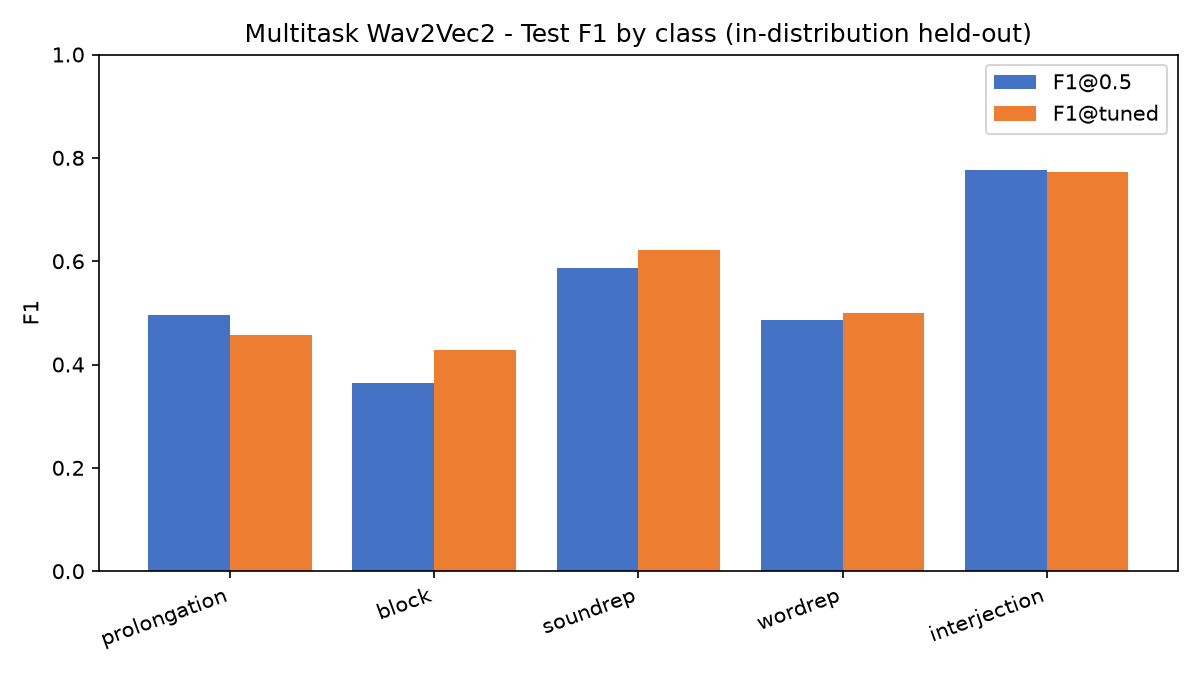
\includegraphics[width=0.85\textwidth]{figures/classifier_test_f1.png}
\Description{Bar chart of per-class F1 scores on the clip-level in-distribution
test set.}
\caption{Per-class F1 scores (multitask Wav2Vec2) on the clip-level
in-distribution test set.}
\label{fig:testf1}
\end{figure}

\begin{figure}[t]
\centering
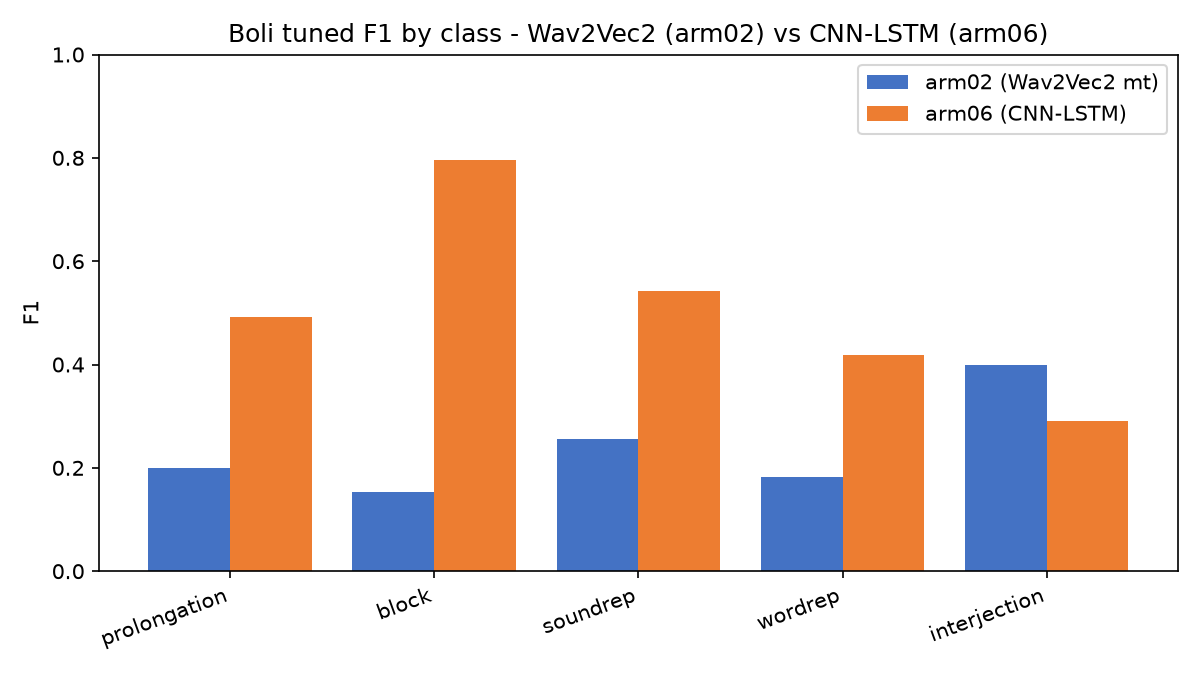
\includegraphics[width=0.85\textwidth]{figures/classifier_boli_f1.png}
\Description{Bar chart of per-class tuned F1 on the Project Boli
speaker-independent cross-corpus held-out set, comparing the shared-backbone
Wav2Vec2 (arm02) and CNN-LSTM (arm06) models.}
\caption{Per-class tuned F1 on the Project Boli speaker-independent
cross-corpus set for the shared-backbone Wav2Vec2 model (arm02) and the CNN-LSTM
model (arm06), each using its per-class validation-F1-optimal thresholds.}
\label{fig:bolif1}
\end{figure}

Under the clip-level in-distribution protocol, the \emph{five-binary Wav2Vec2
classifier} (arm01) achieves the highest measured test macro F1 (0.5704 at tuned
thresholds), and the \emph{multitask Wav2Vec2} with
3-epoch backbone freezing (arm02) follows closely (0.5557)
while using ${\approx}4.9\times$ fewer parameters
than five independent classifiers. The margin between the two top configurations is
only ${\approx}0.015$. Because every configuration is a single training run, this
difference is within the range of run-to-run variation we would expect from
different random seeds, and we do not interpret it as evidence that one
architecture is better than the other; both substantially outperform the remaining
configurations under this protocol.

Backbone-freezing duration matters: the \emph{multitask Wav2Vec2 with 20-epoch
freezing} (arm03) performs notably worse (test F1 $= 0.141$ at default, 0.378 at
tuned), confirming that excessive backbone freezing prevents the model from
learning task-specific representations.

Under the clip-level protocol, the CNN-based configurations (arms04--07) achieve
substantially lower in-distribution macro F1 (0.149--0.269 at default thresholds),
reflecting the limited capacity of small convolutional networks
(${\sim}$300K--540K parameters) relative to the 94M-parameter Wav2Vec2 backbone.
For reference, an all-positive baseline and a base-rate-random classifier achieve
macro F1 of 0.247 and 0.143 on the same test set: the Wav2Vec2 configurations
clearly capture in-distribution signal, while the CNN configurations exceed these
trivial baselines only marginally (tuned macro F1 $0.25$--$0.27$).

\subsection{Speaker-Independent Evaluation (Project Boli)}
On the 53-clip Boli set---whose speakers, languages, and recording conditions are
fully unseen during training---a naive \emph{all-positive} classifier, which
predicts every clip as positive for every dysfluency type, achieves a macro F1 of
$0.550$, \emph{higher than every configuration we evaluated} (best: arm06,
$0.5077$). Table~\ref{tab:boli_perclass} reports per-class tuned F1 for all seven
configurations together with the all-positive baseline. Read naively, the table
appears to show that the CNN configurations ``generalize best'' to the unseen
corpus; however, none of them exceeds the trivial baseline, and the per-class
picture shows why. The CNN configurations reach comparatively high F1 on block,
word repetition, and interjection almost entirely by predicting (nearly) every
clip as positive: at its validation-tuned thresholds, arm06 applies the
positive label to essentially all $53$ Boli clips for block, word repetition, and
interjection, so its per-class
F1 approaches---and for interjection exactly equals---the all-positive F1 that is
achievable without any learning (Table~\ref{tab:boli_thresholdfree}). By contrast, the Wav2Vec2 configurations collapse
toward \emph{all-negative} predictions on the shifted distribution: their macro
predicted-positive rate (PPR) is $0.08$--$0.10$ against an average class base
rate of $0.41$, so their F1 is limited by near-zero recall on most classes. The
tuned-F1 ``reversal'' reported in the in-distribution section
(Table~\ref{tab:macro}) is therefore an artifact of operating-point drift under
distribution shift, not evidence of a difference in generalization ability.

\begin{table}[t]
\caption{Per-class tuned F1 on the Project Boli speaker-independent held-out set
(PR = prolongation, BL = block, SR = sound repetition, WR = word repetition,
IN = interjection). Class support on Boli is small (PR: 16, BL: 35, SR: 34,
WR: 14, IN: 9). ``All-positive'' labels every clip as positive for every class.}
\label{tab:boli_perclass}
\centering
\small
\begin{tabular}{lrrrrrr}
\hline
Arm & PR & BL & SR & WR & IN & Macro\\
\hline
arm01\_5x\_w2v2 & 0.400 & 0.250 & 0.256 & 0.125 & 0.429 & 0.292\\
arm02\_mt\_frz3 & 0.200 & 0.154 & 0.256 & 0.182 & 0.400 & 0.238\\
arm03\_mt\_frz20 & 0.200 & 0.233 & 0.182 & 0.182 & 0.273 & 0.214\\
arm04\_cnn\_pool & 0.308 & 0.491 & 0.182 & 0.387 & 0.290 & 0.332\\
arm05\_cnn\_single & 0.326 & 0.765 & 0.508 & 0.431 & 0.348 & 0.476\\
arm06\_cnn\_lstm & 0.492 & 0.795 & 0.542 & 0.418 & 0.290 & 0.508\\
arm07\_cnn\_tf & 0.316 & 0.320 & 0.490 & 0.267 & 0.333 & 0.345\\
\hline
All-positive & 0.464 & 0.795 & 0.782 & 0.418 & 0.290 & 0.550\\
\hline
\end{tabular}
\end{table}

\begin{table}[t]
\caption{Threshold-free macro metrics and predicted-positive rate (PPR) on the
Project Boli set (53 clips). AUPRC of a random classifier equals the average base
rate (macro $0.408$), so the ``lift'' column reports AUPRC relative to that
prior. PPR is the mean over classes of the fraction of clips predicted positive at
the validation-tuned thresholds.}
\label{tab:boli_thresholdfree}
\centering
\small
\begin{tabular}{lrrrr}
\hline
Arm & Macro AUROC & Macro AUPRC & AUPRC lift & Macro PPR\\
\hline
arm01\_5x\_w2v2 & 0.620 & 0.546 & 1.34 & 0.079\\
arm02\_mt\_frz3 & 0.621 & 0.557 & 1.37 & 0.102\\
arm03\_mt\_frz20 & 0.538 & 0.443 & 1.09 & 0.204\\
arm04\_cnn\_pool & 0.473 & 0.412 & 1.01 & 0.574\\
arm05\_cnn\_single & 0.497 & 0.445 & 1.09 & 0.615\\
arm06\_cnn\_lstm & 0.522 & 0.419 & 1.03 & 0.879\\
arm07\_cnn\_tf & 0.500 & 0.412 & 1.01 & 0.438\\
\hline
\textbf{Base rate (random)} & 0.500 & 0.408 & 1.00 & 0.408\\
\hline
\end{tabular}
\end{table}

The threshold-free metrics corroborate this reading. Table~\ref{tab:boli_thresholdfree}
reports macro AUROC and macro AUPRC for all configurations. The two
task-adapted Wav2Vec2 configurations (arm01, arm02) rank Boli clips best: macro
AUROC $0.620$--$0.621$, and macro AUPRC $0.546$--$0.557$, i.e., a lift of
${\approx}1.3$--$1.4\times$ over the base-rate prior. The frozen-backbone variant
(arm03) sits near chance (AUROC $0.538$, lift $1.09$). The CNN configurations
rank around chance: macro AUROC $0.473$--$0.522$ and macro AUPRC
$0.412$--$0.445$ (lift ${\approx}1.01$--$1.09$). In absolute terms the Wav2Vec2
ranking advantage is modest (e.g., macro AUROC $0.621$ vs.\ $0.522$; each class
has at most 35 positive clips, nine in the worst case), so no strong
generalization claim is warranted in either direction; but the direction of the
evidence is the \emph{opposite} of the F1-based reading: under threshold-free
metrics the Wav2Vec2 models separate dysfluent from fluent clips on the unseen
corpus better than the CNN models do, and none of the seven configurations comes
close to reliable cross-corpus detection.

The primary open question is therefore not ``which representation family
generalizes better''---the present data do not support a CNN advantage once base
rates and operating points are accounted for---but \emph{why}
validation-calibrated operating points drift so strongly under distribution shift,
and whether the modest ranking advantage of Wav2Vec2 features persists on larger
external corpora. We frame two candidate explanations, both of which the present
experiments support only circumstantially and do not directly test:
\begin{itemize}
\item \emph{Operating-point drift hypothesis:} the shifted Boli distribution
changes the models' score distributions (score matching on out-of-domain inputs),
so fixed validation-tuned thresholds land in degenerate regions of the ROC curve.
Because F1 depends on the operating point, it then tracks base rates and the
predicted-positive rate rather than discrimination; threshold-free metrics are
immune to this effect.
\item \emph{Corpus-specificity / spectrogram-invariance hypothesis (ranking):}
the higher-capacity Wav2Vec2 representations may encode corpus-specific
characteristics of SEP-28K/UCLASS---speakers, accents, recording
conditions---that transfer only weakly to unseen speakers and languages, while
the coarse spectral patterns preserved by mel-spectrogram CNNs transfer more
evenly; this would explain why the two families differ in ranking quality the
observed direction without resolving which family is preferable for a given
deployment.
\end{itemize}

Both hypotheses can be tested experimentally without retraining the classifiers:
lightweight \emph{probe} classifiers trained on the frozen embeddings of each
model family---one predicting speaker identity and one predicting the source
corpus---would test the corpus-specificity and spectrogram-invariance hypotheses,
while recalibrating thresholds on a handful of Boli clips would directly quantify
operating-point drift. We leave these probe experiments to future work. The Boli
evaluation set is small (53 clips; per-class support as low as 9), so
definitive conclusions about cross-corpus generalization require additional
external corpora.

\subsection{Per-Class Analysis}
Detailed per-class metrics for the multitask Wav2Vec2 (arm02) on the clip-level
test set at tuned thresholds are presented in Table~\ref{tab:perclass}, including
AUPRC. The tuned thresholds themselves are listed in Table~\ref{tab:thresholds};
for the multitask model these are per-class validation-F1-optimal operating
points (prolongation 0.55, block 0.35, sound repetition 0.40, word repetition
0.35, interjection 0.45). Figure~\ref{fig:testauc} shows the per-class AUROC and
AUPRC.

\begin{table}[t]
\caption{Per-class metrics for the multitask Wav2Vec2 (arm02) on the clip-level
test set at tuned thresholds. Macro is the unweighted mean over classes.}
\label{tab:perclass}
\centering
\footnotesize
\setlength{\tabcolsep}{4pt}
\begin{tabular}{lrrrr}
\hline
Class & F1 (tuned) & AUROC & AUPRC & Support\\
\hline
Prolongation & 0.457 & 0.845 & 0.491 & 400\\
Block & 0.429 & 0.768 & 0.444 & 553\\
Sound Rep. & 0.621 & 0.878 & 0.624 & 494\\
Word Rep. & 0.499 & 0.855 & 0.550 & 366\\
Interjection & 0.773 & 0.935 & 0.848 & 834\\
\hline
\textbf{Macro} & \textbf{0.556} & \textbf{0.856} & \textbf{0.592} & ---\\
\hline
\end{tabular}
\end{table}

\begin{table}[t]
\caption{Per-class validation-tuned thresholds (F1-optimal over the swept grid)
for the multitask Wav2Vec2 (arm02).}
\label{tab:thresholds}
\centering
\small
\begin{tabular}{lr}
\hline
Class & Threshold\\
\hline
Prolongation & 0.55\\
Block & 0.35\\
Sound Rep. & 0.40\\
Word Rep. & 0.35\\
Interjection & 0.45\\
\hline
\end{tabular}
\end{table}

\begin{figure}[t]
\centering
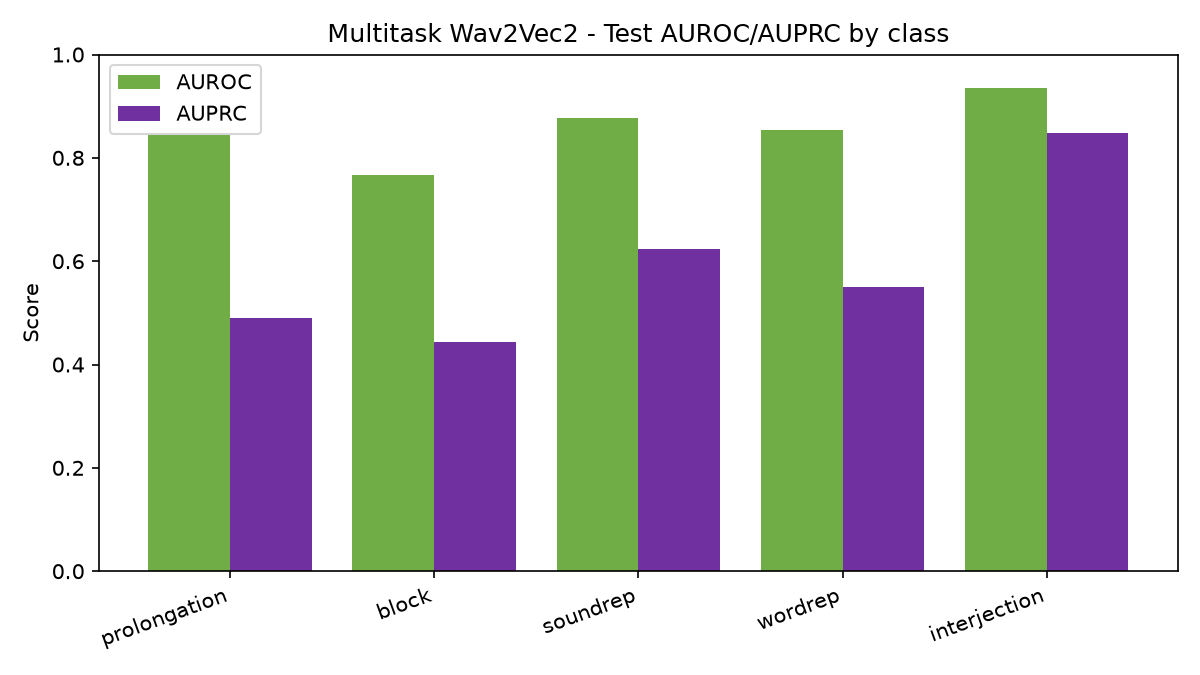
\includegraphics[width=0.85\textwidth]{figures/classifier_test_auc.png}
\Description{Bar chart of per-class area under the ROC curve (AUROC) and
precision-recall curve (AUPRC) on the clip-level test set.}
\caption{Per-class AUROC and AUPRC (multitask Wav2Vec2) on the clip-level test
set.}
\label{fig:testauc}
\end{figure}

Several observations follow.
\begin{itemize}
\item \emph{Interjection} achieves the highest F1 among the evaluated classes
(F1 $= 0.773$, AUROC $= 0.935$, AUPRC $= 0.848$). Filler words (``um,'' ``uh,''
``like'') have distinct acoustic signatures that are well-separated from fluent
speech, making them relatively easy for the model to identify.
\item \emph{Block} is the most challenging class (F1 $= 0.429$, AUROC $= 0.768$,
AUPRC $= 0.444$). Silent pauses and tense pauses before speech are acoustically
similar to normal speech pauses, making them difficult to distinguish without
contextual information. The fixed 3-s window and silence trimming described in
Section~\ref{sec:arch} may additionally suppress the very pause that defines a
block when it falls near a window boundary.
\item \emph{Sound repetition} achieves the second-highest F1 (0.621) with the
second-highest recall (0.627), indicating the model is effective at catching sound
repetitions but with lower precision.
\item The gap between AUROC and F1 (e.g., prolongation AUROC $= 0.845$ vs.\ F1 $=
0.457$) indicates that the model ranks dysfluent clips well but its probability
outputs are not well matched to the validation-tuned operating thresholds when
those thresholds are applied to the test set. We do not measure calibration
directly; quantifying predictive calibration (e.g., expected calibration error and
Brier score, following Guo et al.~\cite{guo2017calibration}) is an explicit item
of future work.
\end{itemize}

Regarding blocks specifically, a natural hypothesis is that explicit temporal and
prosodic features---pause duration, voicing, and energy trajectory around the
suspected pause---would improve block detection beyond what the raw classifiers
extract. We regard this as the most promising single-class improvement and propose
it as a dedicated follow-up study; the present work only isolates the failure
pattern.

Table~\ref{tab:confmat} reports confusion matrices (TP, FP, TN, FN at tuned
thresholds) for the five binary Wav2Vec2 classifiers (arm01) on the test set, and
Figure~\ref{fig:confmat} shows them graphically. They show the same pattern as the
multitask model: interjection is detected most confidently, block produces the
most false negatives and the largest number of false positives relative to its
support, and prolongation is the next most frequently missed.

\begin{table}[t]
\caption{Confusion matrices (TP, FP, TN, FN) for the five binary Wav2Vec2
classifiers (arm01) on the clip-level test set at tuned thresholds. Each row sums
to the 3,715 scored clips.}
\label{tab:confmat}
\centering
\footnotesize
\begin{tabular}{lrrrrr}
\hline
Class & TP & FP & TN & FN & Threshold\\
\hline
Prolongation & 189 & 139 & 3176 & 211 & 0.550\\
Block & 210 & 284 & 2878 & 343 & 0.500\\
Sound Rep. & 301 & 185 & 3036 & 193 & 0.450\\
Word Rep. & 182 & 151 & 3198 & 184 & 0.400\\
Interjection & 668 & 175 & 2706 & 166 & 0.500\\
\hline
\end{tabular}
\end{table}

\begin{figure}[t]
\centering
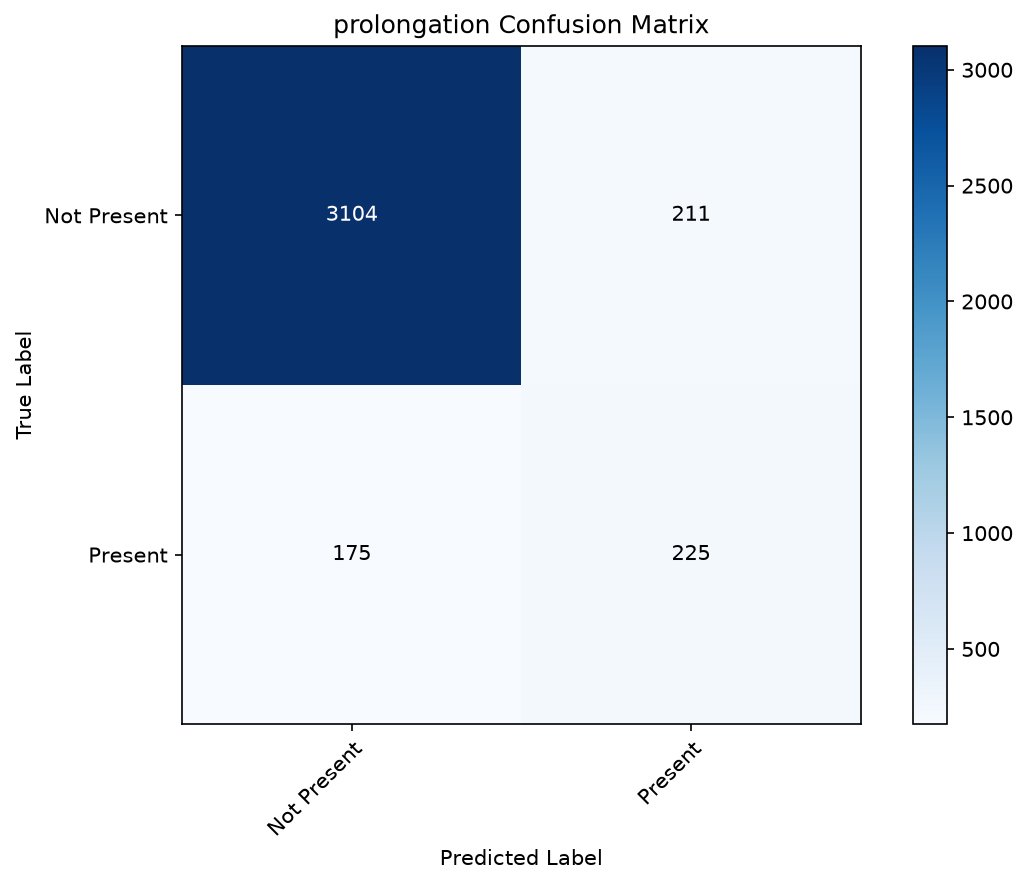
\includegraphics[width=0.31\textwidth]{figures/prolongation_confusion_matrix.png}
\hfill
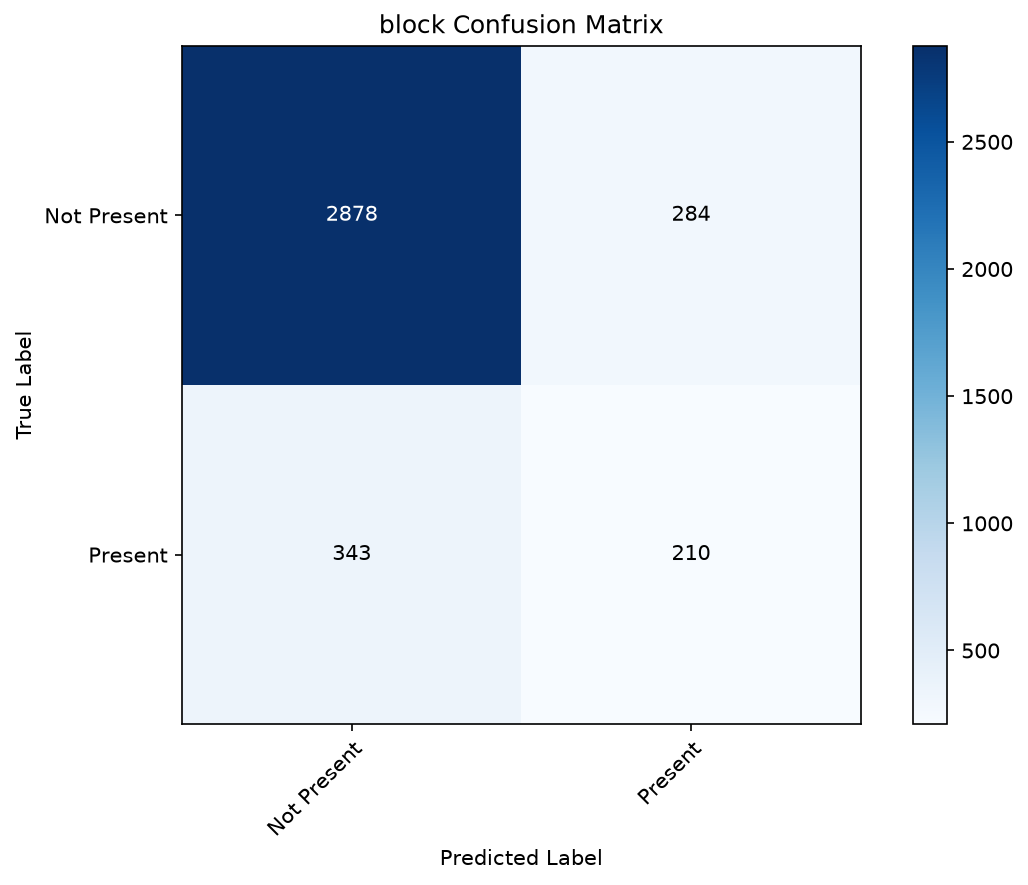
\includegraphics[width=0.31\textwidth]{figures/block_confusion_matrix.png}
\hfill
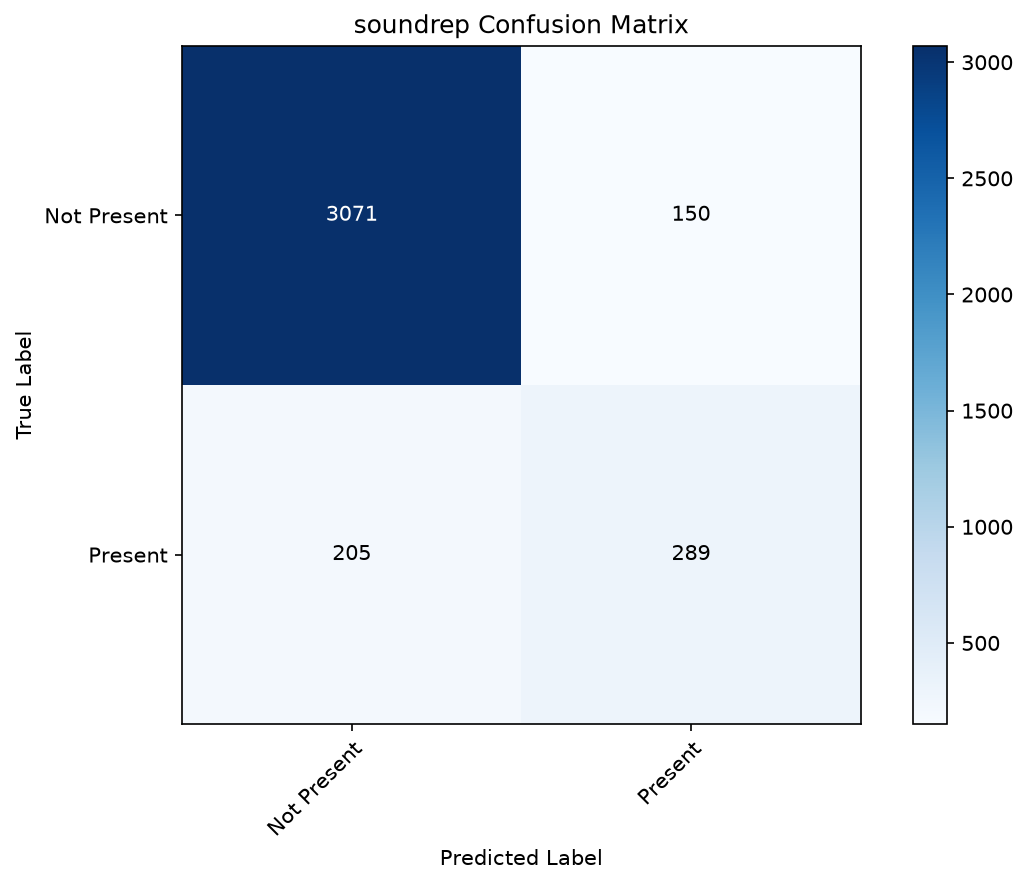
\includegraphics[width=0.31\textwidth]{figures/soundrep_confusion_matrix.png}\\[0.5em]
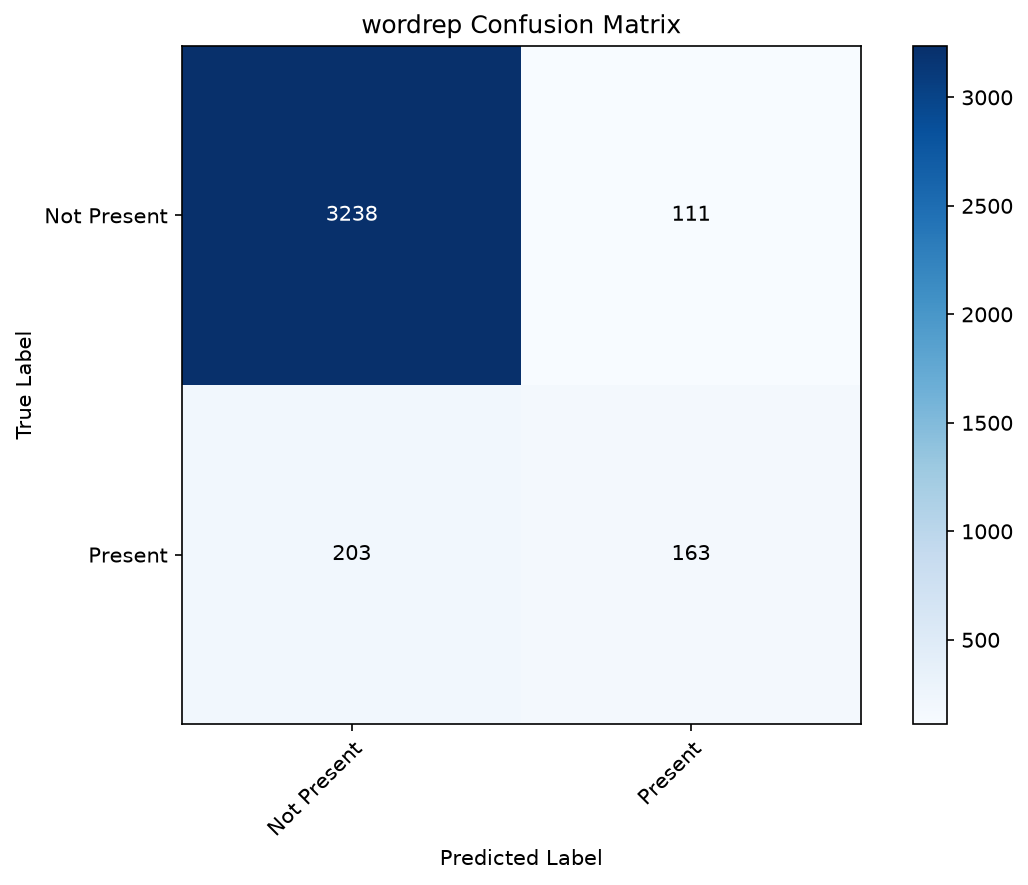
\includegraphics[width=0.31\textwidth]{figures/wordrep_confusion_matrix.png}
\hfill
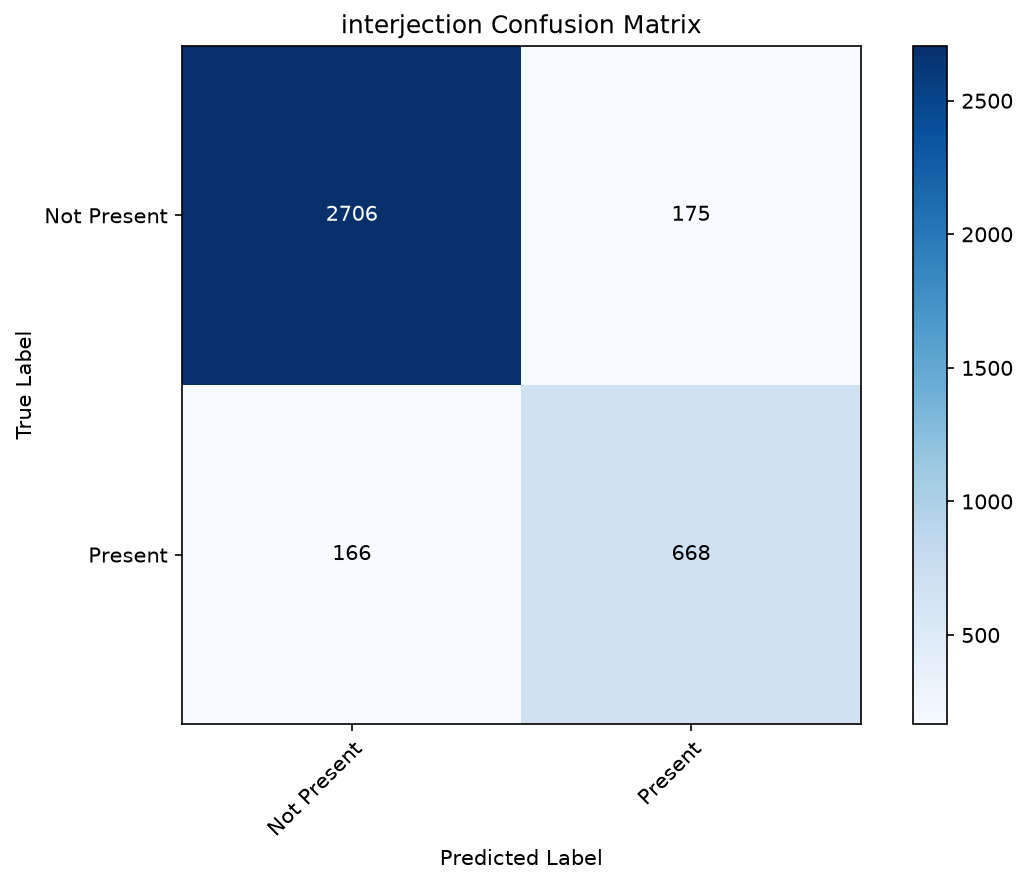
\includegraphics[width=0.31\textwidth]{figures/interjection_confusion_matrix.png}
\Description{Five confusion matrices, one per dysfluency type, for the binary
Wav2Vec2 classifiers on the clip-level in-distribution test set.}
\caption{Confusion matrices for the five binary Wav2Vec2 classifiers (arm01) on
the clip-level in-distribution test set. Top row: prolongation, block, and sound
repetition; bottom row: word repetition and interjection.}
\label{fig:confmat}
\end{figure}

\subsection{Computational Considerations}
Table~\ref{tab:tradeoff} summarizes the parameter-accuracy-generalization
trade-off for the most informative configurations. Sizes are computed from the
reported parameter counts assuming 32-bit floating-point storage
($\text{MB} = \text{params} \times 4 / 10^6$); we did not benchmark GPU memory,
latency, or throughput, and report only the analytically derived footprint.

\begin{table}[t]
\caption{Trade-off between parameter count, computed fp32 size, and evaluation
performance (tuned F1, Table~\ref{tab:macro}). On Boli, an all-positive baseline
reaches macro F1 $0.550$, above every configuration shown here
(Section~\ref{sec:results}).}
\label{tab:tradeoff}
\centering
\small
\begin{tabular}{lrrrr}
\hline
Model family & Params & Size (fp32) & Test F1 & Boli F1\\
\hline
Wav2Vec2 (5$\times$ binary) & 472.8M & 1.89 GB & 0.570 & 0.292\\
Wav2Vec2 (multitask) & 97.3M & 389 MB & 0.556 & 0.238\\
CNN (best) & 540K & 2.2 MB & 0.271 & 0.508\\
\hline
\end{tabular}
\end{table}

Wav2Vec2 models achieve ${\sim}2\times$ higher in-distribution F1 than the CNN
models but comprise roughly 180$\times$ (multitask) to 875$\times$ (five binary
classifiers) more parameters. On the external Boli set their tuned F1 is lower,
but Section~\ref{sec:results} shows that this reflects operating-point drift and
class-base-rate effects rather than a ranking advantage: under threshold-free
metrics the Wav2Vec2 configurations rank Boli clips \emph{better} than the CNNs
(macro AUPRC $0.546$--$0.557$ vs.\ $0.412$--$0.445$). From an engineering
standpoint, the multitask Wav2Vec2 configuration delivers nearly the same
clip-level F1 as five independent classifiers at a fraction of the parameter
budget. The CNN models remain attractive for resource-constrained settings given
their very small footprint, but they are not a drop-in generalization remedy: none
of the evaluated configurations exceeds a trivial baseline on the external
corpus, so cross-corpus deployment of any of these systems is not yet supported
by evidence.

\subsection{Comparison with Published Results}
Our best Wav2Vec2 results (macro F1 $= 0.570$ at tuned thresholds for the
five-binary configuration, 0.556 for the multitask variant, clip-level
split) sit within the range reported in the literature: Bayerl et
al.~\cite{bayerl2022multi} reported macro F1 of 0.56--0.63 on FluencyBank, and
Su\v{s}ac et al.~\cite{susac2026stuttmil} reported per-class F1 from 0.30
(block) to 0.78 (interjection) on SEP-28K with an attention-based
multiple-instance-learning model. Our per-class values follow the same
ordering, with interjection highest (0.773 for the multitask variant) and block
lowest (0.429); our
measured orderings are consistent with that of Su\v{s}ac et al.---for example, our
block F1 is lower than our interjection F1, and both are in the same relative
arrangement. However, differences in datasets, splits, label definitions,
threshold strategies, and evaluation protocols prevent direct attribution of
absolute differences to architecture alone, and we make no such claim.

\subsection{Limitations}
\begin{itemize}
\item \emph{Clip-level in-distribution split:} The test set shares speakers with
training for SEP-28K and UCLASS, inflating in-distribution metrics; those results
are not speaker-independent. The only speaker-independent evidence is the Boli
cross-corpus set, which is small (53 clips).
\item \emph{Single seed:} All results are single training runs from seed 42.
Statistics such as mean $\pm$ standard deviation or confidence intervals require
multi-seed runs and are not available; accordingly we do not claim statistically
significant differences, especially between arm01 and arm02, whose measured
difference (0.014) is small.
\item \emph{Small external corpus:} Boli provides 53 scored clips, with per-class
supports of at most 35; the cross-corpus conclusions are therefore noisy.
\item \emph{Operating-point dependence:} All tuned-F1 results depend on
validation-F1-optimal thresholds. On Boli these thresholds drift strongly (PPR
ranges from 0.08 for the Wav2Vec2 configurations to 0.88 for the CNN
configurations), and no configuration exceeds an all-positive baseline (macro F1
$0.550$) on that set. Cross-corpus \emph{deployment} of any evaluated system is
therefore not supported; threshold-free ranking is reported alongside tuned F1
for this reason.
\item \emph{Untested hypotheses:} The corpus-specificity, spectrogram-invariance,
and operating-point-drift explanations are not directly tested; embedding-based
probe experiments (speaker-ID and source-corpus classifiers) and threshold
recalibration probes are proposed as future work.
\item \emph{Scope of baselines:} Only Wav2Vec2-based and compact CNN models are
evaluated. Additional self-supervised backbones (HuBERT, XLS-R, WavLM), a
classical acoustic baseline (e.g., MFCC + SVM), and further external corpora would
strengthen the comparison and are left to future work.
\item \emph{Calibration:} Predictive calibration (e.g., ECE, Brier score) is not
measured; per-class thresholds are tuned on validation only and may not transfer to
all deployment scenarios.
\end{itemize}

\subsection{Practical Implications}
The results indicate that model selection cannot be grounded in in-distribution
metrics alone: the threshold-dependent F1 ranking reverses on the unseen corpus
through operating-point drift rather than through a real ranking advantage, and
no configuration exceeds a trivial baseline on the external set. Until
speaker-independent evidence is obtained with additional corpora and multiple
seeds, deployment guidance should remain conservative:
\begin{itemize}
\item \emph{Report both protocols and both metric families always:} clip-level
in-distribution and cross-corpus metrics should be reported together, and
threshold-dependent metrics (F1) should be accompanied by threshold-free metrics
(AUROC, AUPRC) and trivial baselines, since any one of these alone under- or
overstates performance.
\item \emph{Inflated-deployment caution:} the in-distribution test shares speakers
with training; any system deployed on new speakers will likely perform below the
reported in-distribution numbers.
\item \emph{Interjection} achieves the highest F1 among the evaluated classes and
can serve as a cheap diagnostic signal, but it should not be equated with
reliability of the remaining classes; block detection in particular requires
complementary signals (e.g., pause-aware features).
\item \emph{Document the split type:} whether speakers overlap between training and
test materially changes how results may be interpreted.
\end{itemize}

% ── VI. CONCLUSION ───────────────────────────────────────────────────
\section{Conclusion}
\label{sec:conclusion}

This paper presented an end-to-end speech dysfluency classification system and
compared seven experimental configurations across two representation families
under a clip-level in-distribution protocol and a speaker-independent cross-corpus
protocol. Our main observations are:
\begin{itemize}
\item Under the clip-level in-distribution protocol, the \emph{five-binary
Wav2Vec2 classifier} achieved the highest measured macro F1 (0.5704), while the
\emph{shared-backbone multitask variant} followed closely (0.5557) using
${\approx}4.9\times$ fewer parameters in total; the difference between the two is
small and should be treated as a single-seed point estimate.
\item On the Project Boli speaker-independent cross-corpus set, no configuration
exceeds an all-positive baseline (macro F1 $0.550$). The apparent F1 advantage of
the CNN configurations is an operating-point artifact---their
validation-calibrated thresholds drift toward near-all-positive predictions
(macro PPR $0.88$) while the Wav2Vec2 thresholds drift toward near-all-negative
(macro PPR $0.08$). Under threshold-free metrics the ranking reverses and becomes
modest: the Wav2Vec2 configurations reach macro AUPRC $0.546$--$0.557$ ($\approx
1.3$--$1.4\times$ the base-rate prior) versus $0.412$--$0.445$ for the CNN
configurations.
\item \emph{Interjection} achieved the highest F1 among the evaluated classes
(0.773), while \emph{block} was the most challenging (0.429), consistent with the
ordering reported elsewhere in the literature.
\item \emph{Backbone freezing duration} materially affects the multitask Wav2Vec2
configuration: freezing for 20 epochs instead of 3 degrades tuned macro F1 by
${\approx}32\%$.
\end{itemize}

The tension between the two protocols---Wav2Vec2 dominating in-distribution and
ranking slightly better on the unseen corpus under threshold-free metrics, yet
suffering far larger operating-point drift---motivates further investigation into
the relationship between representation capacity, corpus-specific information
encoded by a representation, and cross-corpus robustness. We specifically propose:
(1) speaker-independent splits of the full corpus with multi-seed runs and
confidence intervals; (2) embedding-based probe experiments
(speaker-identification and source-corpus classification) together with threshold
recalibration probes to test the corpus-specificity, spectrogram-invariance, and
operating-point-drift hypotheses; (3) additional external corpora and languages;
(4) evaluation of HuBERT, XLS-R, and WavLM backbones as well as a classical MFCC
baseline; (5) quantitative calibration analysis and pause-aware features for block
detection.

% ── BIBLIOGRAPHY ─────────────────────────────────────────────────────
\begin{credits}
\subsubsection{\discintname}
The authors have no competing interests to declare that are relevant to the
content of this article.
\end{credits}
%
% ---- Bibliography ----
%
% BibTeX users should specify bibliography style 'splncs04'.
% References will then be sorted and formatted in the correct style.
%
\bibliographystyle{splncs04}
\bibliography{references}
%
\end{document}